% file: mindmap-bottom-align.tex
% See: https://tex.stackexchange.com/q/444236/23098 (Align the bottom nodes of mindmap)

\documentclass[tikz]{standalone}

\usetikzlibrary{mindmap, positioning}

\begin{document}
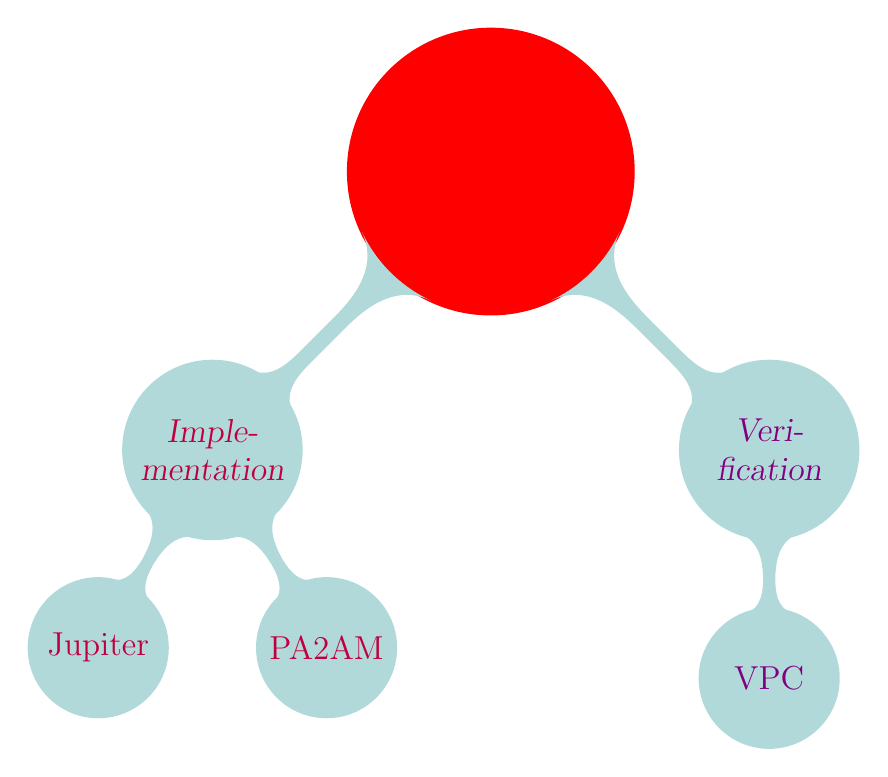
\begin{tikzpicture}[
    root concept/.append style = {concept color = teal!30, sibling angle = 90, font = \LARGE, minimum size = 0pt},
    level 1 concept/.append style = {concept color = teal!30, sibling angle = 90, font = \large},
    level 2 concept/.append style = {concept color = teal!30, sibling angle = 60, font = \large},
  ] 
  \path[mindmap]
    node (spec) [concept, red] {\textsl{Specification}}
    [counterclockwise from = 225]

    child[purple] {
      node[concept] {\textsl{Imple\-mentation}}
      [counterclockwise from = 240]
      child { node (cjupiter) [concept, font = \large] {Jupiter} }
      child { node (pa2am) [concept, font = \large] {PA2AM} }
    }
    child[violet] {
      node (veri) [concept] {\textsl{Veri\-fication}}
      [clockwise from = -90]
      child { node (vpc) [concept, font = \large] {VPC} }
    };
\end{tikzpicture}
\end{document}
